\documentclass[11pt]{article}
\usepackage[letterpaper,margin=1in]{geometry}
\usepackage[T1]{fontenc}
\usepackage{mathpazo}
\usepackage{amsmath,amssymb}
\usepackage{graphicx}
\usepackage{booktabs}
\usepackage{enumitem}
\usepackage{xcolor}
\usepackage[hidelinks]{hyperref}
\usepackage{natbib}
\usepackage[labelsep=period,font=small]{caption}
\setlist{nosep,itemsep=3pt}
\setlength{\parskip}{4pt}
\graphicspath{{../figures/}}
% written by analysis/paper_numbers.py, do not edit
\newcommand{\IRmissfactor}{2.5}
\newcommand{\IRworstmiss}{+27\%}
\newcommand{\MMworstmiss}{0.022}
\newcommand{\ascmBD}{$-$1\%}
\newcommand{\ascmIRa}{$-$23\%}
\newcommand{\ascmIRb}{$-$18\%}
\newcommand{\ascmIRc}{$-$70\%}
\newcommand{\ascmKZ}{$-$14\%}
\newcommand{\ascmMM}{$-$57\%}
\newcommand{\ascmPK}{+8\%}
\newcommand{\ascmSD}{$-$42\%}
\newcommand{\ascmTZ}{+1\%}
\newcommand{\bdIRa}{+2\%}
\newcommand{\bdIRb}{$-$15\%}
\newcommand{\bdSDa}{$-$25\%}
\newcommand{\bdSDb}{$-$11\%}
\newcommand{\bdmBD}{0.0}
\newcommand{\bdmIRa}{0.0}
\newcommand{\bdmIRb}{0.0}
\newcommand{\bdmIRc}{3.4}
\newcommand{\bdmKZ}{0.0}
\newcommand{\bdmMM}{22.7}
\newcommand{\bdmPK}{0.0}
\newcommand{\bdmSD}{1.5}
\newcommand{\bdmTZ}{0.0}
\newcommand{\chancemax}{41\%}
\newcommand{\chancemin}{12\%}
\newcommand{\chinaratio}{5.2}
\newcommand{\chinaratioraw}{5.5}
\newcommand{\confBD}{0.789}
\newcommand{\confIRa}{0.091}
\newcommand{\confIRb}{0.100}
\newcommand{\confIRc}{0.045}
\newcommand{\confKZ}{0.333}
\newcommand{\confMM}{0.167}
\newcommand{\confPK}{0.643}
\newcommand{\confSD}{0.125}
\newcommand{\confTZ}{0.458}
\newcommand{\confhiIRc}{$-$65\%}
\newcommand{\confloIRc}{$-$79\%}
\newcommand{\confminBD}{0.053}
\newcommand{\confminIRa}{0.091}
\newcommand{\confminIRb}{0.050}
\newcommand{\confminIRc}{0.045}
\newcommand{\confminKZ}{0.111}
\newcommand{\confminMM}{0.167}
\newcommand{\confminPK}{0.071}
\newcommand{\confminSD}{0.125}
\newcommand{\confminTZ}{0.042}
\newcommand{\confnIRc}{22}
\newcommand{\cthreebeta}{1.39}
\newcommand{\cthreedepth}{1.25}
\newcommand{\cthreefull}{1.45}
\newcommand{\cthreefullhi}{1.74}
\newcommand{\cthreefulllo}{1.15}
\newcommand{\cthreehi}{1.67}
\newcommand{\cthreelo}{1.10}
\newcommand{\cthreewidth}{0.57}
\newcommand{\cthreewindow}{1.48}
\newcommand{\cthreewindowhi}{1.77}
\newcommand{\cthreewindowlo}{1.18}
\newcommand{\cthreewithout}{0.53}
\newcommand{\cthreewithouthi}{1.41}
\newcommand{\cthreewithoutlo}{$-$0.34}
\newcommand{\cthreewithoutse}{0.45}
\newcommand{\ctwo}{$-$29\%}
\newcommand{\ctwoeq}{$-$26\%}
\newcommand{\ctwohi}{$-$22\%}
\newcommand{\ctwolo}{$-$37\%}
\newcommand{\ctwowithout}{$-$14\%}
\newcommand{\ctwowithoutp}{$p = 0.021$}
\newcommand{\devIR}{+1.0\%}
\newcommand{\discSDa}{$-$62\%}
\newcommand{\discSDb}{$-$64\%}
\newcommand{\discSDse}{0.79}
\newcommand{\discTG}{+41\%}
\newcommand{\discTGdays}{87}
\newcommand{\discUA}{$-$24\%}
\newcommand{\discUG}{$-$26\%}
\newcommand{\discexam}{15}
\newcommand{\discn}{26}
\newcommand{\dosebeta}{1.31}
\newcommand{\doseboothi}{1.53}
\newcommand{\dosebootlo}{1.03}
\newcommand{\dosedayshi}{1.48}
\newcommand{\dosedayslo}{1.15}
\newcommand{\doseflat}{1.02}
\newcommand{\dosehi}{1.56}
\newcommand{\doseinfluence}{89\%}
\newcommand{\doseintercept}{0.015}
\newcommand{\doseinterceptse}{0.071}
\newcommand{\doselo}{1.06}
\newcommand{\dosesancgrowth}{1.16}
\newcommand{\dosesanctwin}{1.28}
\newcommand{\dosewithout}{1.26}
\newcommand{\dosewithoutse}{0.38}
\newcommand{\durmddone}{0.37}
\newcommand{\durmddonewithout}{1.07}
\newcommand{\durmddzero}{0.37}
\newcommand{\durpower}{64\%}
\newcommand{\ethbiggest}{3}
\newcommand{\exposureIRa}{2\%}
\newcommand{\exposurePK}{14\%}
\newcommand{\flatIR}{$-$59\%}
\newcommand{\flatabsIR}{59\%}
\newcommand{\fvpdiff}{$-$0.11}
\newcommand{\fvpmdd}{0.27}
\newcommand{\fvpse}{0.10}
\newcommand{\fvpsize}{5.6\%}
\newcommand{\holmBD}{1.000}
\newcommand{\holmIRa}{0.664}
\newcommand{\holmIRb}{0.664}
\newcommand{\holmIRc}{$<$0.001}
\newcommand{\holmKZ}{1.000}
\newcommand{\holmMM}{$<$0.001}
\newcommand{\holmPK}{1.000}
\newcommand{\holmSD}{0.015}
\newcommand{\holmTZ}{1.000}
\newcommand{\holmpermIRc}{0.084}
\newcommand{\holmpermMM}{0.150}
\newcommand{\holmpermSD}{0.150}
\newcommand{\holmpermmin}{0.084}
\newcommand{\holmpermothers}{0.45}
\newcommand{\jumpBY}{+3\%}
\newcommand{\jumpCU}{+12\%}
\newcommand{\jumpRU}{$-$2\%}
\newcommand{\jumpVE}{+48\%}
\newcommand{\jumpdev}{+9\%}
\newcommand{\jumpearlyhi}{9\%}
\newcommand{\jumpearlylo}{0\%}
\newcommand{\jumpmedian}{+30\%}
\newcommand{\jumpperdev}{+20\%}
\newcommand{\jumpshare}{74\%}
\newcommand{\loomaxmove}{0.18}
\newcommand{\ncIL}{$-$23\%}
\newcommand{\ncILp}{$p = 0.071$}
\newcommand{\ncallowed}{2}
\newcommand{\ncn}{10}
\newcommand{\ncrej}{0}
\newcommand{\ncwidthmax}{105}
\newcommand{\ncwidthmin}{30}
\newcommand{\ndonors}{106}
\newcommand{\nkioexcluded}{24}
\newcommand{\noisebigpfifty}{1.1\%}
\newcommand{\noisebigpninetyfive}{47\%}
\newcommand{\noisesmallpninetyfive}{79\%}
\newcommand{\npool}{82}
\newcommand{\ooniIRbdays}{13}
\newcommand{\ooniIRdays}{49}
\newcommand{\ooniIRshare}{54\%}
\newcommand{\ooniJan}{18}
\newcommand{\ooniMar}{31}
\newcommand{\orgBD}{$-$10.5\%}
\newcommand{\orgIR}{$-$5.1\%}
\newcommand{\orgMM}{$-$3.8\%}
\newcommand{\orgfallbase}{1.3\%}
\newcommand{\outdevIRc}{$-$6.4\%}
\newcommand{\outdevMM}{$-$11.7\%}
\newcommand{\outdevSD}{$-$2.3\%}
\newcommand{\outorgIRc}{$-$8.8\%}
\newcommand{\outorgMM}{$-$8.2\%}
\newcommand{\outorgSD}{$-$3.8\%}
\newcommand{\outrepoIRc}{$-$9.4\%}
\newcommand{\outrepoMM}{$-$19.3\%}
\newcommand{\outrepoSD}{$-$5.2\%}
\newcommand{\permIRc}{0.009}
\newcommand{\permMM}{0.019}
\newcommand{\permSD}{0.019}
\newcommand{\permminp}{0.0093}
\newcommand{\plausible}{33\%}
\newcommand{\plausiblelog}{0.40}
\newcommand{\poolhiIRc}{$-$61\%}
\newcommand{\poolhiMM}{$-$44\%}
\newcommand{\poolhiSD}{$-$16\%}
\newcommand{\poolloIRc}{$-$75\%}
\newcommand{\poolloMM}{$-$64\%}
\newcommand{\poolloSD}{$-$44\%}
\newcommand{\poolpIRc}{0.012}
\newcommand{\poolpMM}{0.012}
\newcommand{\poolpSD}{0.024}
\newcommand{\poolpctIRc}{$-$69\%}
\newcommand{\poolpctMM}{$-$55\%}
\newcommand{\poolpctSD}{$-$32\%}
\newcommand{\rankBY}{14}
\newcommand{\rankCU}{6}
\newcommand{\rankRU}{3}
\newcommand{\repoIR}{$-$4.5\%}
\newcommand{\repoMM}{$-$14.2\%}
\newcommand{\repofallbase}{0.9\%}
\newcommand{\sancgrowthIR}{$-$64\%}
\newcommand{\sanctwinIR}{$-$68\%}
\newcommand{\scBD}{+6\%}
\newcommand{\scIRa}{$-$24\%}
\newcommand{\scIRb}{$-$20\%}
\newcommand{\scIRc}{$-$70\%}
\newcommand{\scKZ}{$-$15\%}
\newcommand{\scMM}{$-$57\%}
\newcommand{\scPK}{+7\%}
\newcommand{\scSD}{$-$38\%}
\newcommand{\scTZ}{+4\%}
\newcommand{\sdidBD}{+11\%}
\newcommand{\sdidIRa}{$-$22\%}
\newcommand{\sdidIRb}{$-$18\%}
\newcommand{\sdidIRc}{$-$69\%}
\newcommand{\sdidKZ}{$-$9\%}
\newcommand{\sdidMM}{$-$56\%}
\newcommand{\sdidPK}{+3\%}
\newcommand{\sdidSD}{$-$32\%}
\newcommand{\sdidTZ}{$-$5\%}
\newcommand{\sdidabsIRc}{69\%}
\newcommand{\sdidhiBD}{+61\%}
\newcommand{\sdidhiIRa}{+7\%}
\newcommand{\sdidhiIRb}{+5\%}
\newcommand{\sdidhiIRc}{$-$61\%}
\newcommand{\sdidhiKZ}{+34\%}
\newcommand{\sdidhiMM}{$-$39\%}
\newcommand{\sdidhiPK}{+29\%}
\newcommand{\sdidhiSD}{$-$13\%}
\newcommand{\sdidhiTZ}{+16\%}
\newcommand{\sdidloBD}{$-$24\%}
\newcommand{\sdidloIRa}{$-$43\%}
\newcommand{\sdidloIRb}{$-$35\%}
\newcommand{\sdidloIRc}{$-$76\%}
\newcommand{\sdidloKZ}{$-$39\%}
\newcommand{\sdidloMM}{$-$69\%}
\newcommand{\sdidloPK}{$-$17\%}
\newcommand{\sdidloSD}{$-$47\%}
\newcommand{\sdidloTZ}{$-$22\%}
\newcommand{\shnormalMM}{4.0\%}
\newcommand{\shnormalSD}{4.5\%}
\newcommand{\shortpool}{$-$7.8\%}
\newcommand{\shortpooldays}{14}
\newcommand{\shortpoolhi}{+5\%}
\newcommand{\shortpoollo}{$-$19\%}
\newcommand{\shortpoolp}{0.214}
\newcommand{\shpermMM}{2.0\%}
\newcommand{\shpermSD}{3.5\%}
\newcommand{\shsims}{200}
\newcommand{\shsmallMM}{4.6\%}
\newcommand{\shsmallSD}{7.9\%}
\newcommand{\simcov}{98\%}
\newcommand{\simpowthirtyfive}{88\%}
\newcommand{\simpowtwenty}{41\%}
\newcommand{\simsize}{1.6\%}
\newcommand{\sizedecades}{2.04}
\newcommand{\sizeest}{0.014}
\newcommand{\sizemdd}{0.19}
\newcommand{\sizemddrange}{0.39}
\newcommand{\sizese}{0.072}
\newcommand{\stackmone}{$-$6\%}
\newcommand{\stackmonep}{$p = 0.217$}
\newcommand{\stackmtwo}{$-$7\%}
\newcommand{\stackmtwop}{$p = 0.134$}
\newcommand{\stackone}{$-$8\%}
\newcommand{\stackonep}{$p = 0.294$}
\newcommand{\stackzero}{$-$31\%}
\newcommand{\stackzerop}{$p<0.001$}
\newcommand{\supn}{30}
\newcommand{\timingjoint}{2.5\times10^{-4}}
\newcommand{\vpnexcess}{1.2}
\newcommand{\vpnmde}{23}
\newcommand{\vpnmissing}{736}
\newcommand{\vpnse}{6.1}
\newcommand{\wikinoisepninetyfive}{40\%}

\renewcommand{\ttdefault}{pcr}
\makeatletter\newcommand{\tabin}[1]{\@@input #1 }\makeatother

\title{Internet shutdowns and the GitHub activity attributed to a country\\[4pt]
\large A synthetic control study of nine shutdowns, 2021 to 2026}
\author{Matin Nikoomanzar\\ \small University of California, Los Angeles}
\date{Working paper, October 2026}

\begin{document}
\maketitle

\begin{abstract}
\noindent When a government cuts off a country's internet, how much of the country's activity on GitHub disappears from GitHub's map? I build a synthetic counterfactual for each of nine shutdowns from \ndonors{} economies that have no shutdown in my event registry, using GitHub's quarterly Innovation Graph. Every estimate is checked against placebos, three estimators, conformal inference, four donor pools, ten crises that came without a shutdown, and two independent daily data sources. Git pushes attributed to Iran in the first quarter of 2026, when the country was offline for about half the quarter, came in at \sdidIRc{} against the counterfactual (95\% interval \sdidloIRc{} to \sdidhiIRc{}), or \flatIR{} if Iran would have missed the jump most economies had that quarter. Iran 2026 passes every check I fixed in advance. Myanmar after its 2021 coup came in at \sdidMM{} and passes every check that can be run on it, though with four quarters of history those checks are weak. Daily OONI test counts, which have nothing to do with GitHub, put Iran's blackout days at \ooniIRdays, inside the 48 to 58 days in my registry. The outcome is activity GitHub places in a country by IP address and says nothing about national output. Activity that moved to a VPN exit country is counted as lost, and the absolute falls in repository and organization counts, which almost never happen, are consistent with that. The earlier claim in this project that ``each day offline cost 1.3 days of work'' does not survive. The slope rests about \doseinfluence{} on one event and drops to \doseflat{} if Iran would not have shared the jump. The four full shutdowns of 11 days or less pool to \shortpool{} (\shortpoollo{} to \shortpoolhi), so they can't be seen in quarterly data.
\end{abstract}

\section{Question}

Governments shut down the internet often, and the people who write software lose their tools along with everyone else. I want to know two things. First, when a country goes offline, how much does the GitHub activity attributed to that country fall compared with what similar economies predict? Second, how much of that fall is real lost work and how much is measurement, meaning activity that keeps happening but gets placed in another country?

The first question can be answered with the data. The second one only partly, and a big part of this paper is about where the line is. The outcome throughout is geographically attributed GitHub activity. It is not productivity, output or employment, and nothing here should be read as a cost of shutdowns to the economy.

This is the second version of the project. The first version estimated the same nine events and reported a ``days of work lost'' headline and a dose response slope of 1.31. Before running anything new, I wrote down which tests would count, how I would correct for running many of them, and what wording each result would earn (Appendix~\ref{app:plan}). Some of the old claims fail those rules, and I say so where it happens.

\section{Data and what it measures}
\label{sec:data}

\paragraph{GitHub Innovation Graph.} GitHub publishes quarterly counts by economy from 2020 \citep{innovationgraph}. I use four. Git pushes count uploads during the quarter, so they are a flow. Developers, repositories and organizations are counts at the end of the quarter and include accounts and projects that are no longer active, so they are close to stocks. The datasheet is specific about location. A developer is placed in the economy their IP address shows on most days of the quarter, the last known location is carried forward on days with no activity, and the whole quarter's activity goes to that one economy. Repositories and organizations are placed by the most common location of their members.

Three things follow. A developer who goes dark during a blackout stays in their country, because the last location is carried forward. A developer who gets online through a VPN for most of the quarter is moved, with all of that quarter's pushes, to the VPN's exit economy. And GitHub itself warns that VPN use distorts the numbers. GitHub's own supplement for 2025 to 2026, which reweights pushes by the location people write in their profiles, puts China's activity at about \chinaratio{} times what IP addresses show, relative to the typical economy among the \supn{} in the file. Iran isn't in that file. So for a country under heavy censorship, attributed activity can sit far below real activity even in normal times, and a shutdown can push more of it out.

I use the pinned commit \texttt{078fb62} of the data repository. When I checked on 20 October 2026, upstream had no newer quarters (the latest is 2026Q1) and all four files were byte for byte the same as my copy (\texttt{data/provenance\_github.json}). The panel keeps the 149 economies with every quarter present. Donors are the \ndonors{} of those with no shutdown in my registry and at least 10,000 pushes in every quarter. That rule is weaker than it sounds, because \nkioexcluded{} of the donors have a full network shutdown in the Access Now data (Section~\ref{sec:falsification}).

\paragraph{Event registry.} \texttt{data/events.csv} lists the nine events with start and end dates, full or partial, which networks were cut, a range for days offline, region and a public source. A validator checks every row (dates inside the headline quarter, day counts that fit the window, https sources) and checks that every pre-2026 event has a record in the Access Now data starting within a week of my date. All nine pass. Iran 2026 is newer than the Access Now release.

\paragraph{Outside data.}
\begin{itemize}
\item Access Now's KeepItOn shutdown tracker for 2020 to 2025 \citep{keepiton}, 1,418 records in 84 countries (CC BY 4.0). I use it to build a donor pool without shutdowns, to check the registry, to pick negative controls, and to find shutdowns my registry doesn't have.
\item OONI daily measurement counts for all 149 economies \citep{ooni} (CC BY-NC-SA 4.0, so the derived columns in the released dataset carry that license). OONI volunteers run network tests from phones and computers, and the count of tests uploaded per day falls toward zero when a country goes dark. It is the main independent daily source here.
\item Wikimedia's daily pageviews by country \citep{wikimedia} (CC0). They start in February 2023 and, for countries on Wikimedia's higher risk list, only in February 2024. Iran and Myanmar are never published. So this source can only check Bangladesh 2024 and Tanzania 2025.
\item Regions from \texttt{country\_converter} and 2020 World Bank income groups via Our World in Data.
\end{itemize}
I looked at GH Archive as a second software source, but its event records carry no location, so there is no sound way to build a country series from it.

\section{Design}
\label{sec:design}

For an event in country $i$ with headline quarters $\mathcal{T}_1$ and clean pre quarters $\mathcal{T}_0$, let $Y_{it}$ be the log of the outcome. A synthetic counterfactual is a weighted mix of donors, $\hat Y_{it}(0) = \hat\mu + \sum_j \hat\omega_j Y_{jt}$, with weights fit on $\mathcal{T}_0$ only. The effect is the average gap over $\mathcal{T}_1$, reported as $e^{\hat\tau}-1$.

I use three estimators. Synthetic difference in differences \citep{arkhangelsky2021} is the headline, as in version 1. It adds a ridge penalty on unit weights and also weights the pre quarters. Synthetic control \citep{abadie2010} in the demeaned form \citep{fermanpinto2021}. Ridge augmented synthetic control \citep{benmichael2021}, which corrects whatever pre period imbalance the weights leave with a ridge regression of donors' later outcomes on their pre period, picking the penalty by leave one out error across donors. All three solve for weights exactly as nonnegative least squares problems.

\paragraph{What has to be true.}
\begin{description}[style=unboxed,leftmargin=0pt]
\item[A1. The twin's path.] Without the shutdown, the treated country would have moved like its weighted mix of donors in the headline quarters. This is the one that matters most and the one I test hardest (Section~\ref{sec:falsification}).
\item[A2. No anticipation.] Nothing changed in the pre quarters because of the coming shutdown. Quarters touched by any other listed event in the same country are dropped from the pre period.
\item[A3. Donors untouched.] The shutdown doesn't change donors' outcomes. VPN reassignment breaks this a little, because activity moved out of Iran lands in donors like Germany or the Netherlands. That pushes the twin up and the estimate down, but the amounts are tiny next to those donors' totals (Section~\ref{sec:measurement}).
\item[A4. Stable measurement.] GitHub's attribution rule and bot filters don't change in a way that hits one country and not its donors.
\end{description}
What I do not assume is that the shutdown was the only thing that happened. Iran's 2026 blackouts came with mass protests after a currency collapse and then with US and Israeli strikes from 28 February \citep{rferl2026, jurist2026}. Myanmar's came with a coup, Sudan's with a coup. So each estimate is the change in attributed activity during everything that happened that quarter, and the negative controls and the dose response are how I try to separate the internet part.

\paragraph{Inference.} The standard error is the larger of two placebo spreads. In space, every donor gets the fake event and the same design. In time, the treated country gets fake events at earlier quarters, which measures how noisy that country is. Version 1's simulations planted 1,500 fake shutdowns and found this interval covers the truth \simcov{} of the time with \simsize{} false alarms, so it is conservative. Those simulations use at least eight quarters before the event and donors with at least 10,000 pushes, so they don't speak for Myanmar (four pre quarters) or Sudan (seven). Confirmatory p values are two sided normal ones from this standard error, corrected across the nine events with Holm. I also report the exact permutation p value and the conformal p value of \citet{cwz2021}, which fits the twin under the null on all quarters and compares post period residuals with every cyclic shift in time. Conformal p values can't go below one over the number of quarters used, which is \confminIRc{} at best here and \confminMM{} for Myanmar.

For those two settings I ran a smaller set of \shsims{} fake events each, copying their number of pre and post quarters (the script is \texttt{short\_history.py}). With Myanmar's shape (four before, two after) the false alarm rate at 5\% is \shnormalMM{} with the normal p value and \shpermMM{} with the permutation p. With Sudan's shape it is \shnormalSD{} and \shpermSD, and \shsmallSD{} when the donors are small (under 10,000 pushes). In both settings there are too few earlier quarters to draw time placebos, so the standard error comes from the donors alone.

One property makes the power work cheap. All three estimators fit weights on the pre period only, so planting an effect $d$ in a post quarter moves the estimate by exactly $d$. A test checks this to machine precision. Simulating a planted effect therefore needs only draws of each event's estimation error, which the placebos already give.

\section{Results}

Table~\ref{tab:main} has every event with every check from the plan. Figure~\ref{fig:iran} shows the clearest one.

\begin{figure}[t]
\centering
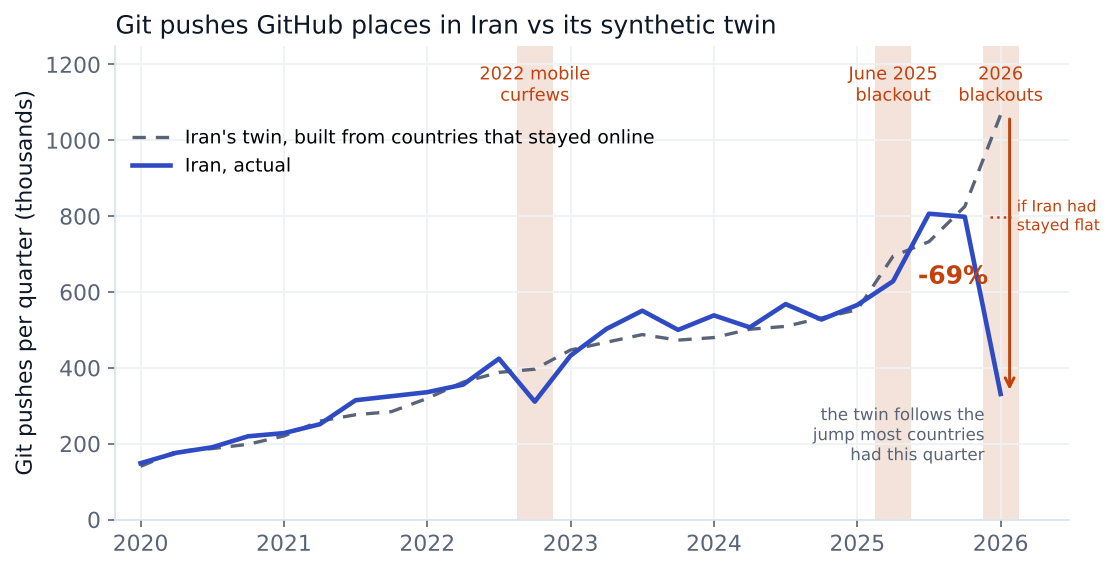
\includegraphics[width=0.92\linewidth]{iran.png}
\caption{Iran against its synthetic counterfactual. The dotted line marks the 2026 outcome if Iran had stayed flat from the quarter before instead of joining the jump most economies had.}
\label{fig:iran}
\end{figure}

\begin{table}[t]
\centering\footnotesize
\setlength{\tabcolsep}{3.5pt}
\resizebox{\linewidth}{!}{%
\begin{tabular}{llrlrrrlllrl}
\toprule
Event & Kind & SDiD & 95\% interval & SC & ASCM & Holm p & Conformal p (floor) & F2 & F3 & Breakdown & Clear \\
\midrule
\tabin{tables/main.tex}
\bottomrule
\end{tabular}}
\caption{Change in attributed git pushes against the twin. F2 is backdating, F3 the donor pools and leave one out. Breakdown is how many times the benchmark miss the twin's path would have to be off before zero enters the interval (Section~\ref{sec:falsification}). ``Clear'' means every check in the plan passed. $^\dagger$ every check that can be run passed, backdating can't be.}
\label{tab:main}
\end{table}

Iran 2026 at \sdidIRc{} passes every check. Myanmar 2021 at \sdidMM{} passes every check that can be run on it. The three estimators agree within a few points for both, and the Holm corrected p values are below 0.001.\footnote{That column takes the placebo spread as roughly normal, as the plan says. The placebo gaps have heavy tails, so I also computed Holm on the exact permutation p. It gives Iran 2026 \holmpermIRc, Myanmar \holmpermMM{} and Sudan \holmpermSD, and \holmpermothers{} or more for the rest. With \ndonors{} donors the smallest permutation p is $1/(\ndonors+1)$, and times nine events that is \holmpermmin, so this version can never fall below it and Iran 2026 sits on that floor. The plan fixed the normal version as the decision rule and listed the permutation p as reported only. The exact p values are $\permIRc$ for Iran 2026 and $\permMM$ for Myanmar, where Ethiopia is the only donor with a larger placebo gap.} Myanmar's twin can't be backdated because it has only four pre quarters, so F2 is ``not testable'' rather than a pass. Under the plan's wording rule that keeps it short of a clear drop, and I treat it as a strong but less tested result. ``Passes every check that can be run'' is weaker than it sounds for Myanmar. Its breakdown value of \bdmMM{} compares against the in-sample fit of those four quarters (a miss of \MMworstmiss{} in logs), which can hardly fail. Its time placebo spread is zero because there are too few earlier quarters to fake events in, so its standard error comes from the donors alone, and its conformal p value sits at the floor of \confMM. The simulations in Section~\ref{sec:design} don't cover its setting, so I ran a smaller set (below).

Sudan 2021 is \sdidSD{} with a Holm p of \holmSD, and all three estimators agree. It fails backdating. Fit without its last two pre quarters, the twin misses them by \bdSDa{} and \bdSDb. Access Now records a nationwide mobile shutdown for school exams from 19 June to 3 July 2021, which is inside those held out quarters, so the twin was probably fit to an already disturbed stretch. Under the plan's rules I can't call it a clear drop.

The other six are not distinguishable from zero after the correction. Iran 2022 (\sdidIRa) and Iran 2025 (\sdidIRb) are the right sign and the right size for their exposure, but their intervals include zero, and Iran 2022 also fails backdating. The four short shutdowns (Kazakhstan, Tanzania, Pakistan, Bangladesh) are what the simulations predict. A drop of 20\%, about 18 days offline, is caught only \simpowtwenty{} of the time.

The precision weighted average over the six full shutdowns is \ctwo{} (95\% \ctwolo{} to \ctwohi), \ctwoeq{} with equal weights, and \ctwowithout{} without Iran 2026 (\ctwowithoutp). That last number is carried by Sudan 2021, which lasted 24 days and fails backdating. The four full shutdowns of 11 days or less (Kazakhstan, Bangladesh, Tanzania and Iran 2025) pool to \shortpool{} (95\% \shortpoollo{} to \shortpoolhi, $p = \shortpoolp$). Pooling doesn't make the short ones visible. It leaves a small effect that I can neither find nor rule out.

\section{Falsification and sensitivity}
\label{sec:falsification}

\begin{figure}[t]
\centering
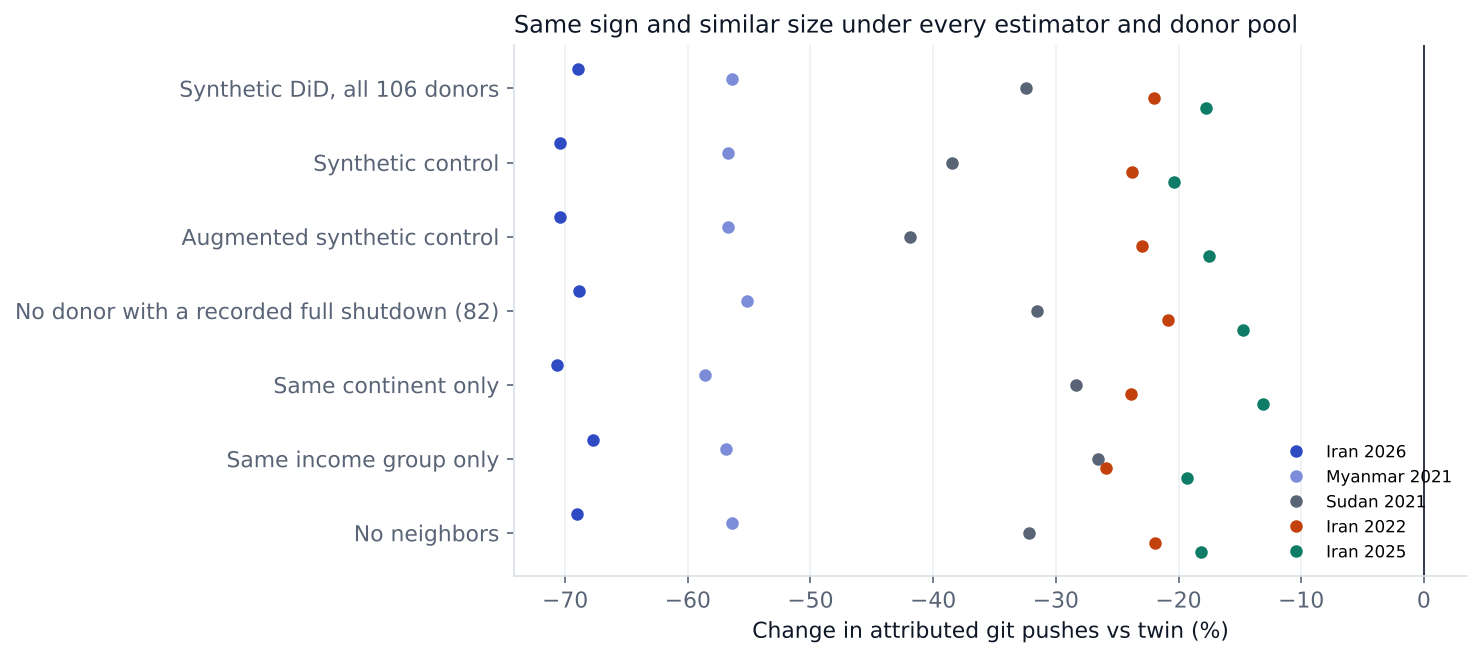
\includegraphics[width=0.85\linewidth]{checks.png}
\caption{The same estimate under each estimator and donor pool.}
\label{fig:checks}
\end{figure}

\paragraph{Donor pools and estimators (F3).} Figure~\ref{fig:checks}. Dropping every donor that had a full network shutdown in the Access Now data (\nkioexcluded{} of \ndonors, including Belarus, Ethiopia, Iraq and Cuba), keeping only the same continent, only the same 2020 income group, or dropping land neighbors moves no estimate by more than one standard error, and only Pakistan's, which is near zero anyway, changes sign. Leaving out each donor with weight over 1\% moves no estimate by more than \loomaxmove{} standard errors.

The plan fixed the full pool as the primary one, so it stays primary, but the \npool{} donors with no full network record deserve a place next to it. There Iran 2026 is \poolpctIRc{} (\poolloIRc{} to \poolhiIRc, permutation p \poolpIRc), Myanmar 2021 is \poolpctMM{} (\poolloMM{} to \poolhiMM, p \poolpMM) and Sudan 2021 is \poolpctSD{} (p \poolpSD). Ethiopia, a donor in the full pool with a 38 day nationwide full network shutdown from 30 June to 6 August 2020, has the largest placebo gap in \ethbiggest{} of the nine windows (Kazakhstan, Myanmar and Pakistan), and it is the only donor with a bigger gap than Myanmar. That is why Myanmar's permutation p is \permMM{} in the full pool and \poolpMM{} in the smaller one.

\paragraph{Backdating (F2).} Holding out the last two pre quarters turns them into real out of sample checks. Iran 2026's twin misses them by \bdIRa{} and \bdIRb, inside the placebo band. Sudan 2021 and Iran 2022 fail, as described above.

\paragraph{Stacked event study.} In a plain synthetic control the pre period gaps sit near zero by construction, so they say little about pre-trends. I refit each event with its last two pre quarters held out and stack them (Figure~\ref{fig:stacked}). Myanmar has no hold-out, and the two held out quarters have eight and seven events. The held out quarters average \stackmtwo{} (\stackmtwop) and \stackmone{} (\stackmonep), the shutdown quarter \stackzero{} (\stackzerop, nine events), and the next quarter \stackone{} (\stackonep). Uncertainty comes from running the identical design on randomly drawn donors. The small negative lead is the thing to watch. It isn't significant, but it is in the direction of a slowdown before the event, which a political crisis would produce.

\begin{figure}[t]
\centering
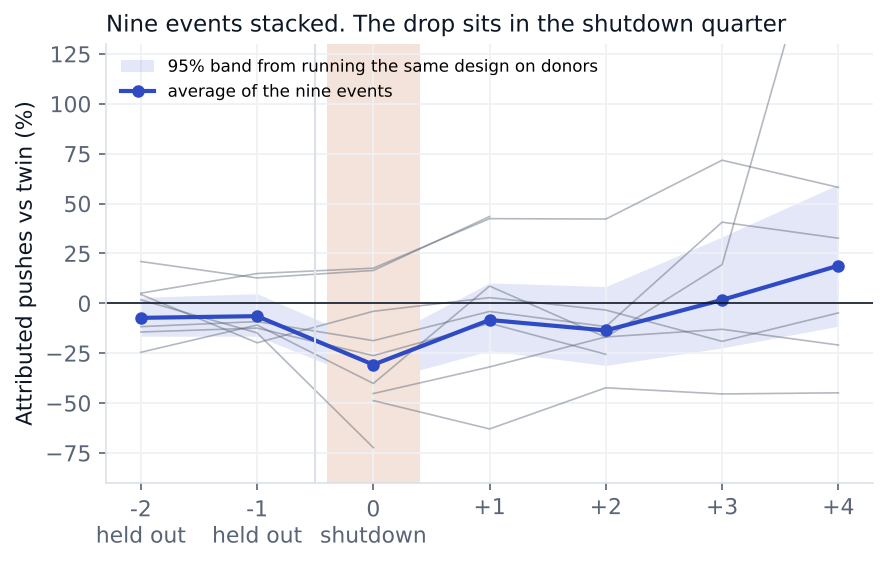
\includegraphics[width=0.66\linewidth]{stacked.png}
\caption{Stacked event study. Grey lines are the nine events, the band comes from the same design run on donors.}
\label{fig:stacked}
\end{figure}

\paragraph{Negative controls (F1).} If crises alone drive the drops, crises without a shutdown should show them too. I picked \ncn{} quarters with a war, natural disaster, economic crisis or protest wave and no full network shutdown in the Access Now data, each with a public source (Table~\ref{tab:controls}, Figure~\ref{fig:controls}). The plan defines the test and the number of rejections allowed but not the list. I chose the ten on 20 October 2026, right after writing the plan and before running them. I searched for major crises from 2021 to 2025 in donor economies and kept those where Access Now has no full network record in that quarter (service blocks only), so the list is mine and was not pre-registered. \ncrej{} of \ncn{} reject at 5\%, against \ncallowed{} allowed by chance, so the check passes. The largest is Israel after 7 October 2023 at \ncIL{} (\ncILp). A war with no shutdown moved attributed activity by about as much as Iran 2022 and Iran 2025. The controls are noisy too, with 95\% intervals \ncwidthmin{} to \ncwidthmax{} points wide, so they only rule out crisis effects as big as the two large drops. Iran 2026 and Myanmar 2021 are more than twice as big as anything in the controls, but the moderate estimates can't be told apart from a crisis effect.

\begin{table}[t]
\centering\small
\begin{tabular}{lllrlr}
\toprule
Economy & Quarter & What happened & vs twin & 95\% interval & p \\
\midrule
\tabin{tables/controls.tex}
\bottomrule
\end{tabular}
\caption{Negative controls. Sources are in \texttt{data/negative\_controls.csv}.}
\label{tab:controls}
\end{table}

\begin{figure}[t]
\centering
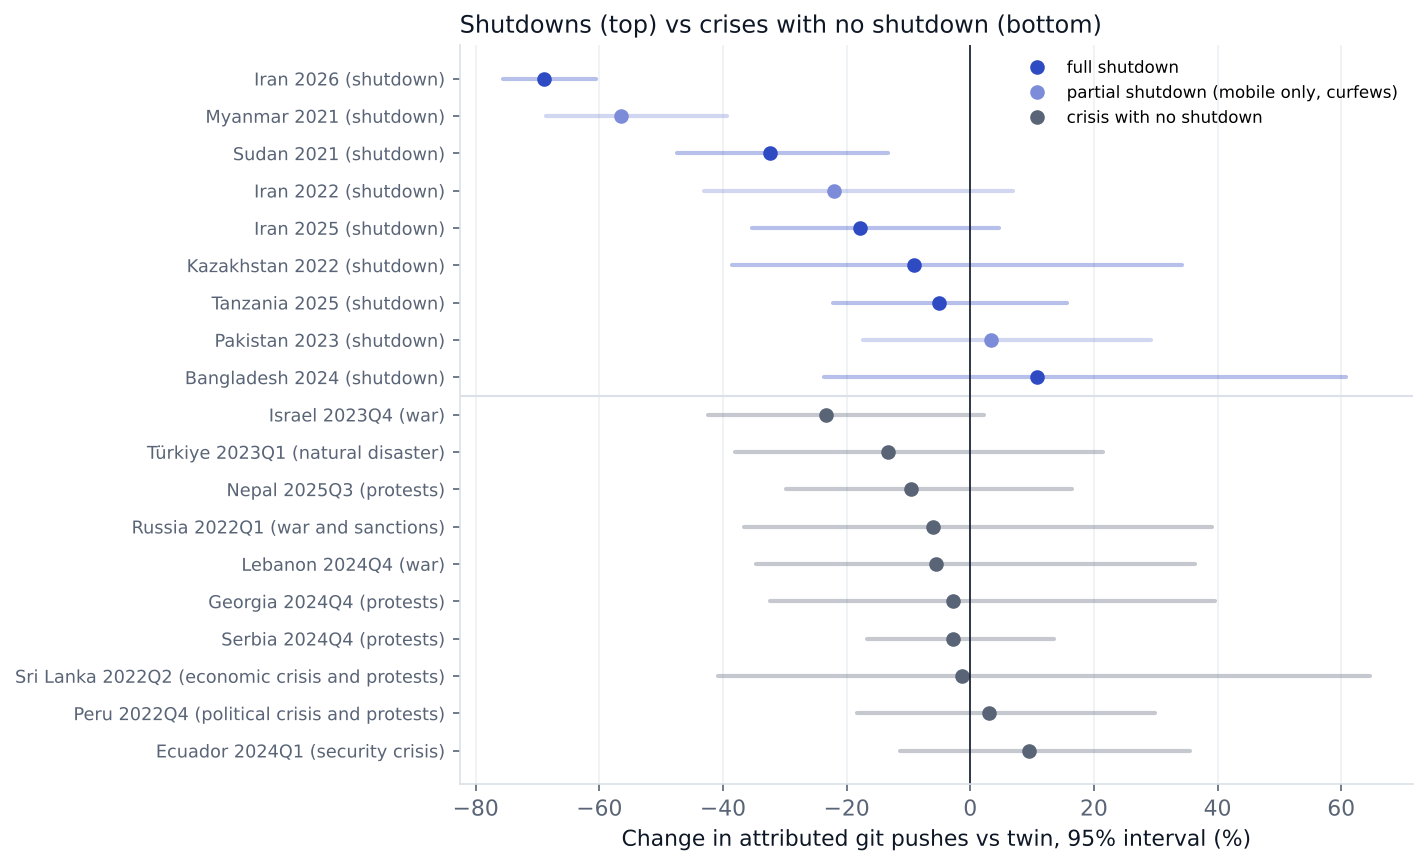
\includegraphics[width=0.8\linewidth]{controls.png}
\caption{Registry shutdowns next to crises with no shutdown.}
\label{fig:controls}
\end{figure}

\paragraph{How big a violation of A1 would erase each result?} In the spirit of \citet{rambachanroth2023} I allow the true counterfactual to drift off the twin by up to $M$ times a benchmark miss, which widens the interval to $\hat\tau \pm (M\cdot\text{miss} + 1.96\,\widehat{se})$. The benchmark is the worst out of sample miss of the twin in the country's own past (the in-time placebos). For Iran that worst miss is \IRworstmiss{}. Iran 2026 survives until $M = \bdmIRc$, so the twin would have to be about \IRmissfactor{} times too high, more than three times the worst miss in Iran's own history. Myanmar and Sudan have too little history, so their benchmark is the in-sample pre fit, which flatters them.

\paragraph{Conformal inference.} The conformal p value for Iran 2026 is \confIRc{}, the smallest possible with \confnIRc{} quarters, with an interval of \confloIRc{} to \confhiIRc. For every other event the test can't reject at 5\% even in principle or doesn't, which says more about how few quarters there are than about the events.

\paragraph{The 2026 jump.} The weakest point of the Iran 2026 number is A1 itself. Most economies' pushes jumped in 2026Q1 (median donor \jumpmedian{} over the quarter before), and Iran's twin jumps with them. Economies under broad sanctions mostly didn't. Russia's pushes changed by \jumpRU, Belarus's by \jumpBY{} and Cuba's by \jumpCU. Venezuela, at \jumpVE, is the exception and sits inside my sanctioned group. In the placebo run for that quarter Russia ranks \rankRU, Cuba \rankCU{} and Belarus \rankBY{} from the bottom of 106. If Iran would also have missed the jump, the change is \flatIR{} with a flat counterfactual and \sancgrowthIR{} if Iran had grown like those economies. A twin built only from them gives \sanctwinIR, with a poor pre fit. I report the Iran 2026 drop as a range from \flatIR{} to \sdidIRc{} for that reason.

What the jump was is unclear. The median donor's pushes rose \jumpmedian{}, but its developers rose only \jumpdev, so most of it is more pushes per developer (\jumpperdev). \jumpshare{} of donors grew by more than 20\%, against median first quarter growth between \jumpearlylo{} and \jumpearlyhi{} in 2021 to 2025. I haven't found a cause and won't guess at one. If it comes from a change in how GitHub counts pushes that reaches Iran differently, that breaks assumption A4.

\section{Measurement}
\label{sec:measurement}

\paragraph{Independent daily timing.} Table~\ref{tab:exposure} and Figure~\ref{fig:ooni}. Using the rule fixed in the plan (a day is disrupted when OONI tests fall below half the median of the 91 days before), OONI shows a run of disrupted days inside the registry window for all five full shutdowns where it has enough tests. In quiet donor quarters a window of the same length and position catches a run by chance \chancemin{} to \chancemax{} of the time, so all five lining up by luck has probability about $\timingjoint$ if the five are treated as independent. Iran 2026 has \ooniIRdays{} disrupted days (\ooniJan{} in January, \ooniMar{} in March), inside the registry's 48 to 58. Wikimedia pageviews, a second independent source, put Bangladesh's cut at 18 to 23 July 2024 and Tanzania's at 29 October to 2 November 2025, matching the registry start dates to the day. There is one disagreement. OONI and Access Now both show Iran's June 2025 disruption starting on 13 June, when the war began, and OONI counts \ooniIRbdays{} days, while my sourced registry entry says 17 June and 7 to 9 days. I kept the registry as sourced and use the OONI numbers as a check. Mobile only shutdowns (Iran 2022, Pakistan 2023) don't show in OONI, which runs on computers too.

\begin{table}[t]
\centering\footnotesize
\setlength{\tabcolsep}{3pt}
\begin{tabular}{llrp{3.6cm}lp{2.2cm}}
\toprule
Event & Registry days & OONI days & OONI runs of 3+ days & In window (chance) & Wikimedia runs \\
\midrule
\tabin{tables/exposure.tex}
\bottomrule
\end{tabular}
\caption{Independent daily checks of each shutdown. Dates are month-day of the headline quarter.}
\label{tab:exposure}
\end{table}

\begin{figure}[p]
\centering
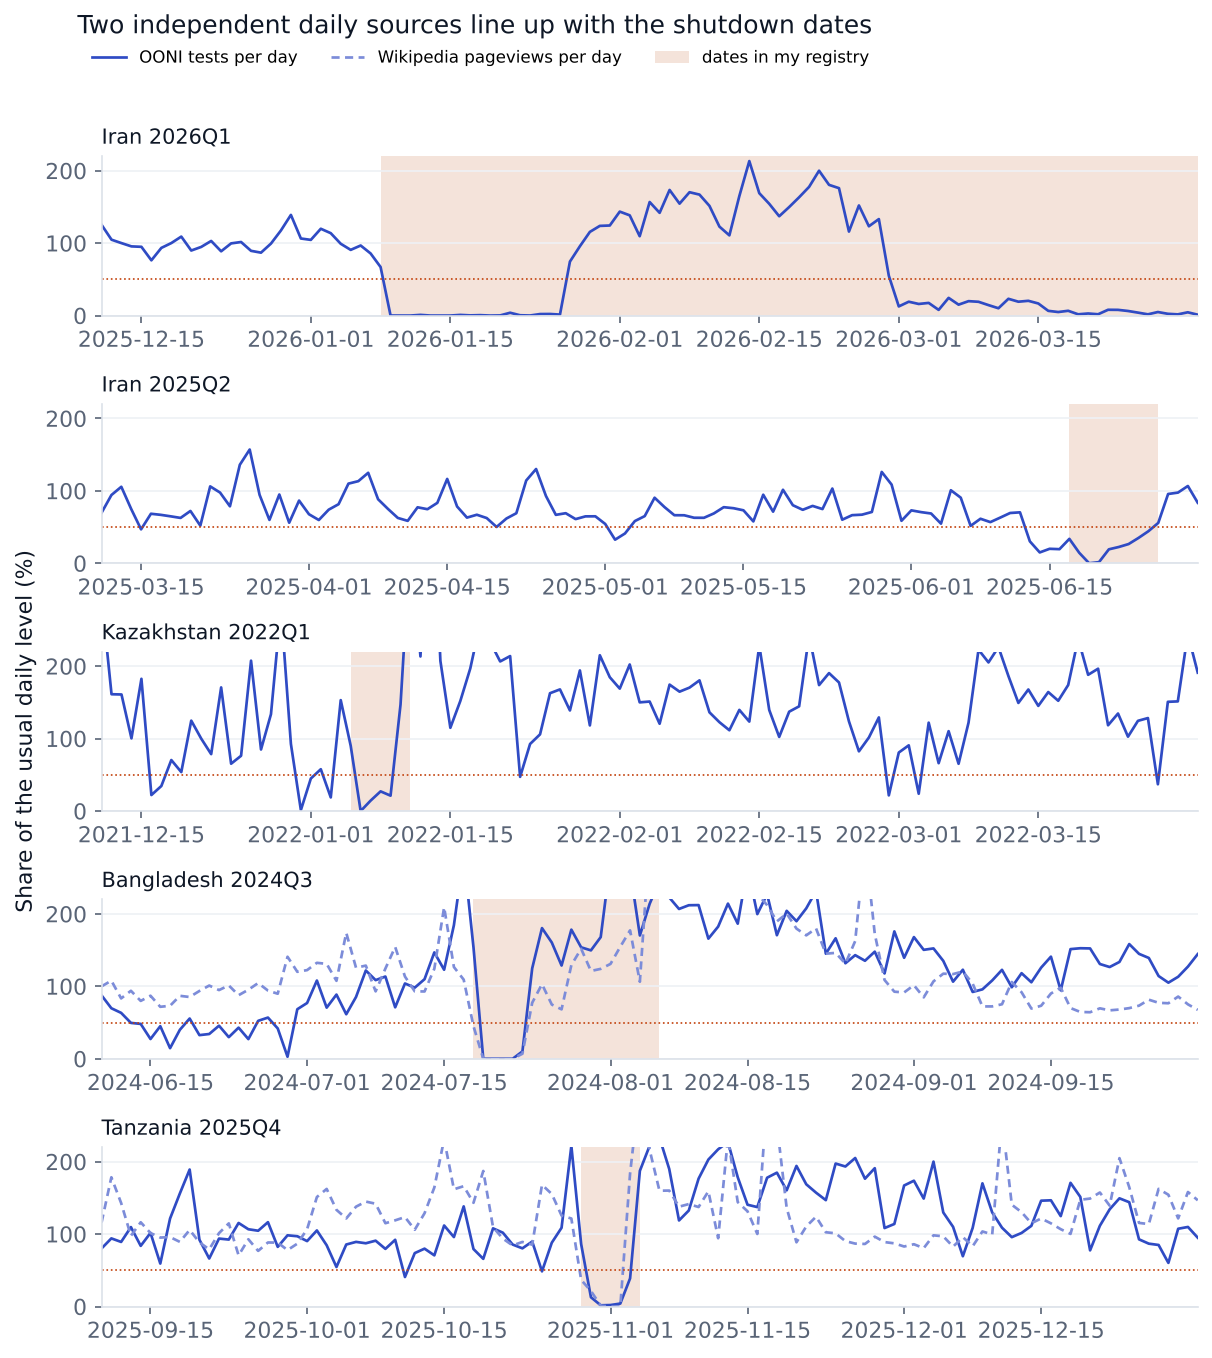
\includegraphics[width=0.9\linewidth]{ooni.png}
\caption{Daily OONI tests and Wikipedia pageviews relative to the usual level, with the registry dates shaded.}
\label{fig:ooni}
\end{figure}

As a measure of how much of a quarter was offline, OONI is weaker than as a calendar. Counts swing when a heavy volunteer starts or stops. In quiet quarters for countries with 5,000 or more tests a day, the share of ``disrupted'' days is \noisebigpfifty{} at the median but \noisebigpninetyfive{} at the 95th percentile, and \noisesmallpninetyfive{} for countries with 100 to 1,000 tests a day. Only Iran 2026, at \ooniIRshare, clearly beats that noise.

\paragraph{Four outcomes.} Table~\ref{tab:outcomes}. For the three events with a significant drop in pushes, all four counts fall against the twin, and for the six without one, nothing does except Bangladesh's organizations. The stocks move much less than pushes, as they should, since they include inactive accounts. The direction agrees everywhere it can be measured.

\begin{table}[t]
\centering\small
\begin{tabular}{lrrrr}
\toprule
Event & Git pushes & Developers & Repositories & Organizations \\
\midrule
\tabin{tables/outcomes.tex}
\bottomrule
\end{tabular}
\caption{Synthetic DiD on all four outcomes. $^*$ p $<$ 0.05.}
\label{tab:outcomes}
\end{table}

\paragraph{A fingerprint of reassignment.} Version 1 said developers ``fell'' 6\% in Iran and 12\% in Myanmar (\outdevIRc{} and \outdevMM{} here). Those were gaps to the twin. In absolute terms Iran's developer count still grew, by \devIR{} in 2026Q1. The more telling numbers are repositories and organizations, which are placed by where their members are seen and include dead projects, so they almost never shrink. Across all economy-quarters, repository counts fall more than 2\% only \repofallbase{} of the time. In 2026Q1 Iran's repositories changed by \repoIR{} and its organizations by \orgIR, the first repository fall in Iran's series. In 2021Q2 Myanmar's repositories changed by \repoMM{} and its organizations by \orgMM. Bangladesh's organizations changed by \orgBD{} in its shutdown quarter. A project doesn't stop existing because its owner is offline. It gets placed somewhere else when its members show up from other IP addresses most days, which is what VPN use would do (Figure~\ref{fig:drift}). The other way a count can fall is GitHub removing or reclassifying projects, which I can't rule out from the outside. So some of the measured drop in pushes is activity that kept happening and was counted elsewhere.

\begin{figure}[t]
\centering
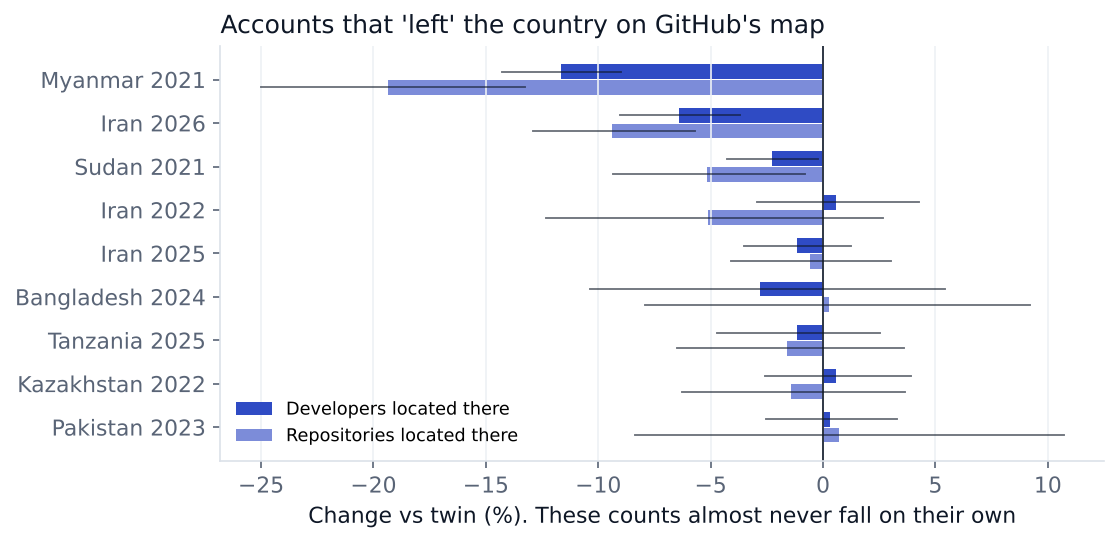
\includegraphics[width=0.75\linewidth]{drift.png}
\caption{Absolute change in repository and organization counts from the quarter before.}
\label{fig:drift}
\end{figure}

\paragraph{Can the moved activity be found? (F4).} I fixed a list of likely VPN exit economies before running this check (the United States, Germany, the Netherlands, the United Kingdom, France, Finland, Sweden, Canada, Singapore, Turkey and the UAE), estimated each one's gap against twins built from the other donors, and added up the excess. Version 1 had already published the Iran 2026 number, so the list was not fixed before I saw that estimate. For Iran 2026 the missing pushes come to about \vpnmissing{} thousand. The exit economies' combined excess is $+\vpnexcess$ million with a standard error of \vpnse{} million, so the smallest reassignment this test could detect is about \vpnmde{} times the whole missing amount. The test has no power. The activity could all be there and I would not see it, which makes this the biggest question the data can't answer.

\section{Dose response and heterogeneity}

\paragraph{Version 1's slope.} Version 1 fit the log effect on $\log(1-s)$, with $s$ the share of the quarter offline, through the origin across the six full shutdowns, and got \dosebeta{} (\doselo{} to \dosehi), read as ``each day offline cost 1.3 days of work''. Taken apart (Figure~\ref{fig:het}), \doseinfluence{} of the fit's weight is Iran 2026. Without it the slope is \dosewithout{} with a standard error of \dosewithoutse. If Iran's counterfactual is flat the slope is \doseflat, and with sanctioned economy growth \dosesancgrowth. Uncertainty in the day counts moves it between \dosedayslo{} and \dosedayshi, and resampling each event's error from its placebos gives \dosebootlo{} to \doseboothi. With an intercept the intercept is \doseintercept{} (se \doseinterceptse), so a zero day shutdown does predict no effect.

\paragraph{With an outside measure of exposure (C3).} Using the OONI share of disrupted days instead of my own day counts, the slope across the seven events where OONI is usable is \cthreebeta{} (\cthreelo{} to \cthreehi). It is positive, which is what C3 tests, so drops do grow with time offline in these data. The plan only allowed me to say anything about a slope of exactly 1 if the interval was narrower than 0.5. It is \cthreewidth{} wide, so I say nothing about it.

Three things weaken even the positive result. Iran 2026 carries it. Without that event the slope is \cthreewithout{} (\cthreewithoutlo{} to \cthreewithouthi). Two of the exposure values are poor. Pakistan 2023 gets \exposurePK{} from OONI, but the disrupted days are in April and the shutdown was 9 to 12 May, so that value is noise from the quiet before the event. Iran 2022 gets \exposureIRa{} because the evening mobile curfews hardly show up in OONI. I checked two fixes. Counting only days inside each event's registry window gives \cthreewindow{} (\cthreewindowlo{} to \cthreewindowhi), and using only the five full shutdowns gives \cthreefull{} (\cthreefulllo{} to \cthreefullhi). Neither moves the slope much. The window version is a deviation from the plan and is listed in Appendix~\ref{app:plan}.

Bigger shares of the quarter offline go with bigger drops in attributed pushes, and that is all the data support. ``Days of work lost'' fails for three reasons. The data can't tell a slope of 1.3 from 1, the measure includes reassigned activity, and the one event that sets the slope also depends on the 2026 jump.

\begin{figure}[t]
\centering
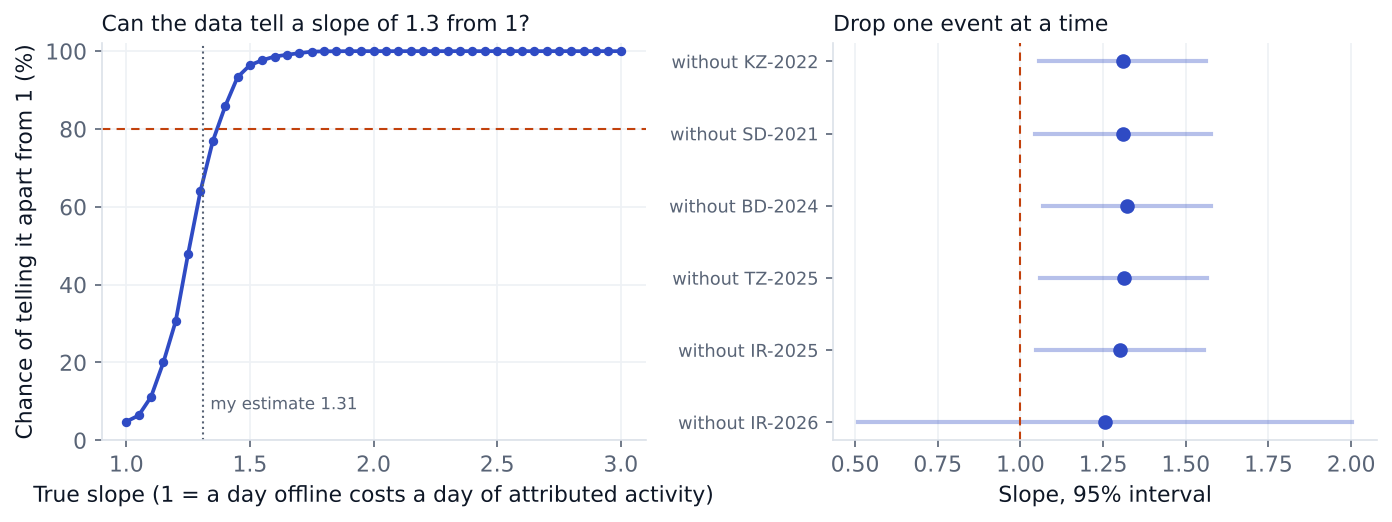
\includegraphics[width=0.95\linewidth]{heterogeneity.png}
\caption{Left, the chance of telling a true slope from 1 with these six events. Right, the slope with each event left out.}
\label{fig:het}
\end{figure}

\paragraph{Can the data answer the heterogeneity questions?} Before reading any difference I simulated the minimum detectable difference at 80\% power, drawing each event's error from its own placebo distribution. I compare it with a plausible difference, the drop a month offline would give at one for one (\plausible, \plausiblelog{} in logs).
\begin{itemize}
\item Duration. The minimum detectable slope against 1 is \durmddone, so a true 1.3 is found only \durpower{} of the time, and without Iran 2026 the minimum detectable difference is \durmddonewithout. The data can't separate a day costing a day from a day costing 1.3 days.
\item Full vs partial. The minimum detectable difference is \fvpmdd{} in logs, under the plausible size, with a size of \fvpsize{} at zero. The estimated difference is \fvpdiff{} (se \fvpse), which is nothing. But the groups mix very different durations (Myanmar's partial event ran for months), so this isn't a clean comparison of kinds of shutdown.
\item Developer base. The minimum detectable slope is \sizemdd{} in logs per tenfold difference in pre period pushes. The events span about \sizedecades{} tenfolds, so that is \sizemddrange{} across the range against a plausible \plausiblelog, which makes the question barely answerable. The estimate is \sizeest{} (se \sizese), with no sign that bigger developer communities lose a different share.
\end{itemize}

\section{Shutdowns my registry doesn't have}

A fixed rule in the Access Now data (nationwide, full network, fixed and mobile both cut, at least five days, panel economy, from 2021) finds all six full shutdowns in my registry from before 2026 and \discn{} other country-quarters, \discexam{} of them exam shutdowns in Iraq, Syria and Algeria. Exam shutdowns last a few hours a day, and none shows a clear drop, which fits. Table~\ref{tab:discovery} has the rest, with the drop the version 1 slope would predict from the day count. Sudan's 2024 wartime shutdown comes out at \discSDa{} and \discSDb{} for its two quarters, in line with the prediction, but Sudan's standard error is \discSDse{} during the war, so it can't test anything. Togo 2025 is the odd one. Access Now codes \discTGdays{} days as full network and service based, and GitHub shows \discTG. Whatever happened, the day count overstates it for GitHub users, which is a reminder that tracker day counts say how long restrictions lasted and nothing about how deep they went.

\begin{table}[t]
\centering\small
\begin{tabular}{llrlrrr}
\toprule
Economy & Quarter & Days & Recorded cause & vs twin & se (log) & Predicted \\
\midrule
\tabin{tables/discovery.tex}
\bottomrule
\end{tabular}
\caption{Non-exam shutdowns found by the rule and not in my registry. Sources are in \texttt{results/discovery.json}.}
\label{tab:discovery}
\end{table}

\section{Limitations}

\begin{itemize}
\item The outcome is GitHub activity placed by IP address. It misses private repositories and everything off GitHub, and it counts VPN users wherever their VPN exits. Some of each drop is reassignment, and I can't measure how much.
\item Each estimate bundles the shutdown with everything else in that quarter. The negative controls show a crisis alone can move attributed activity by \ncIL{} (Israel 2023), so only the two large events are clearly more than that.
\item Iran 2026 depends on whether Iran would have joined the 2026 jump, whose cause I haven't found. The answer moves the estimate from \sdidIRc{} to \flatIR.
\item The donor pool has \nkioexcluded{} economies with a full network shutdown in the Access Now data. The pool without them gives about the same answers for the large events.
\item Quarterly data can't see shutdowns shorter than about a month one at a time. The four full shutdowns of 11 days or less pool to \shortpool{} (\shortpoollo{} to \shortpoolhi), which is neither a detection nor a rule out.
\item Myanmar has four pre quarters and Sudan seven, so their twins rest on little history, Myanmar can't be backdated, and their breakdown values use a weaker benchmark that can hardly fail. Their standard errors come from the donors alone. The short history simulations put false alarms near \shnormalMM{} for Myanmar's setting and \shnormalSD{} for Sudan's.
\item OONI counts are noisy outside large countries, and Wikimedia covers only two of the events.
\item Nobody independent has reviewed this yet.
\end{itemize}

\section{Reproducibility}

{\sloppy Everything in this paper comes from code in the repository. \texttt{make all} rebuilds every result, figure, report card, the released dataset and this paper from the committed data in a few minutes. \texttt{make sims} reruns the planted shutdown simulations (about 25 minutes), and \texttt{make data} downloads every outside source again. The raw GitHub clone and the Access Now spreadsheet are not in the repository and are fetched into \texttt{data/external} (or the folder in \texttt{SHUTDOWNS\_EXTERNAL}) when needed. The MIT license covers the code only, and the data keeps the licenses listed in Section~\ref{sec:data}. Every number in the text is written into \texttt{paper/numbers.tex} by \texttt{analysis/paper\_numbers.py}, so none is typed by hand. The estimators are tested on simulated panels with known effects, including placebo test size under the null and the exact shift property, and the registry is validated by tests. \texttt{shutdowns estimate} runs the full design on any economy and quarter and writes a one page report card.\par}

\bibliographystyle{plainnat}
\begin{thebibliography}{99}
\bibitem[Abadie et~al.(2010)]{abadie2010} Abadie, A., Diamond, A. and Hainmueller, J. (2010). Synthetic control methods for comparative case studies. \emph{Journal of the American Statistical Association} 105(490), 493-505.
\bibitem[Arkhangelsky et~al.(2021)]{arkhangelsky2021} Arkhangelsky, D., Athey, S., Hirshberg, D., Imbens, G. and Wager, S. (2021). Synthetic difference in differences. \emph{American Economic Review} 111(12), 4088-4118.
\bibitem[Ben-Michael et~al.(2021)]{benmichael2021} Ben-Michael, E., Feller, A. and Rothstein, J. (2021). The augmented synthetic control method. \emph{Journal of the American Statistical Association} 116(536), 1789-1803.
\bibitem[Chernozhukov et~al.(2021)]{cwz2021} Chernozhukov, V., W\"uthrich, K. and Zhu, Y. (2021). An exact and robust conformal inference method for counterfactual and synthetic controls. \emph{Journal of the American Statistical Association} 116(536), 1849-1864.
\bibitem[Ferman and Pinto(2021)]{fermanpinto2021} Ferman, B. and Pinto, C. (2021). Synthetic controls with imperfect pretreatment fit. \emph{Quantitative Economics} 12(4), 1197-1221.
\bibitem[Rambachan and Roth(2023)]{rambachanroth2023} Rambachan, A. and Roth, J. (2023). A more credible approach to parallel trends. \emph{Review of Economic Studies} 90(5), 2555-2591.
\bibitem[GitHub(2026)]{innovationgraph} GitHub (2026). GitHub Innovation Graph, datasheet version 1.0.10. \url{https://github.com/github/innovationgraph}
\bibitem[Access Now(2026)]{keepiton} Access Now (2026). KeepItOn STOP data, 2016 to 2025. \url{https://www.accessnow.org/keepiton-data/}
\bibitem[OONI(2026)]{ooni} Open Observatory of Network Interference. Measurement aggregation API. \url{https://api.ooni.io}
\bibitem[Wikimedia(2026)]{wikimedia} Wikimedia Foundation. Differentially private daily pageviews by country. \url{https://analytics.wikimedia.org/published/datasets/country_project_page/}
\bibitem[RFE/RL(2026)]{rferl2026} Radio Free Europe/Radio Liberty (2026). Iran internet blackout after US and Israeli military attack. \url{https://www.rferl.org/a/iran-internet-blackout-us-israel-military-attack/33690399.html}
\bibitem[JURIST(2026)]{jurist2026} JURIST (2026). Rights group decries Iran internet blackout amid nationwide protest. \url{https://www.jurist.org/news/2026/01/rights-group-decries-iran-internet-blackout-amid-nationwide-protest}
\end{thebibliography}

\appendix
\section{Analysis plan}
\label{app:plan}
% analysis plan, written 20 October 2026 before any of the new checks were run.
% this file is input by both analysis_plan.tex (standalone) and paper.tex (appendix).

I wrote this plan on 20 October 2026, before running any of the checks below. One honest caveat first. The nine event estimates in the first version of this project (synthetic DiD on git pushes, 106 donors) were already public when I wrote it, so they are not pre-registered in the strict sense. What the plan fixes in advance is everything new: which tests are confirmatory, how I correct for running many of them, what counts as a failed falsification check, and what wording the README is allowed to use. If a later run breaks a rule here, the write up says so instead of quietly changing the rule.

\paragraph{Question.} When a government cuts off a country's internet, how much does the GitHub activity that GitHub attributes to that country fall, compared with what similar economies predict? And how much of any fall is measurement (activity that keeps happening but gets placed in another country) rather than less work? The outcome is not national output or productivity. GitHub places a developer in the country their IP address shows on most days of the quarter, so everything here is about geographically attributed GitHub activity.

\paragraph{Fixed design.}
\begin{itemize}
\item Primary outcome: log git pushes per quarter. Secondary: log developers, log repositories, log organizations. These three are end of quarter counts that include inactive accounts, so they mostly measure where accounts are placed and how many new ones appear. I expect them to move much less than pushes and will not call a small move a contradiction.
\item Primary estimator: synthetic difference in differences with the same windows and donor rule as version 1 (no listed shutdown, at least 10,000 pushes in every quarter). Secondary: demeaned synthetic control and ridge augmented synthetic control.
\item Events: the nine in \texttt{data/events.csv}, unchanged. Events found later in outside data (Access Now, OONI) are reported separately and never join the confirmatory family.
\item Exposure (how much of the quarter was offline) comes from OONI daily measurement counts, which have nothing to do with GitHub. Baseline is the median daily count over the 91 days before the event's first quarter. A day is disrupted when its count is below half the baseline. Exposure is the share of disrupted days in the quarter. Only countries with a baseline of at least 100 measurements a day are used. Sensitivity thresholds are 25\% and 75\%.
\end{itemize}

\paragraph{Confirmatory tests.}
\begin{description}
\item[C1.] For each of the nine events, the null is no change in attributed pushes in the headline quarters. The p value is two sided from the placebo standard error (the larger of the in-space and in-time placebo spreads), which the simulations show is calibrated or conservative. Holm correction across the nine at a 5\% family error rate. The exact in-space permutation p value and the conformal p value of Chernozhukov, W\"uthrich and Zhu (2021) are reported but decide nothing.
\item[C2.] Pooled effect: the precision weighted average over the six full shutdowns, with uncertainty from redrawing each event's estimation error from its own placebo distribution. Null is zero.
\item[C3.] Dose response: across events where OONI exposure is measurable, the slope of the log effect on $\log(1-\text{exposure})$ is positive (one sided). Whether the slope is exactly 1 (``a day offline costs a day'') is exploratory, and I only say something about it if the 95\% interval for the slope is narrower than 0.5.
\end{description}

\paragraph{Falsification checks, pass or fail fixed in advance.}
\begin{description}
\item[F1.] Negative controls: economies with a big crisis, protest wave or new sanctions in a quarter but no full network shutdown in the Access Now data for that quarter, each with a cited public source. Passes if the number of controls with $p<0.05$ is no more than a Binomial$(n, 0.05)$ gives 95\% of the time.
\item[F2.] Backdating: refit each event with its last two pre quarters held out. Passes if the held out gaps sit inside the 95\% placebo band.
\item[F3.] Donor pools: (a) donors with no full network shutdown of any kind in the Access Now data for 2020 to 2025, (b) donors on the same continent, (c) donors in the same World Bank income group in 2020, (d) all donors except land neighbors, (e) leave one donor out for every donor with weight above 1\%. Passes if the sign never flips and the estimate never moves by more than one standard error.
\item[F4.] VPN reassignment: if people in a blacked out country keep pushing through VPNs, GitHub should place that activity in the exit country. I fixed the list of likely exit economies before looking at any 2026 numbers. They are the big hosting markets: United States, Germany, Netherlands, United Kingdom, France, Finland, Sweden, Canada, Singapore, Turkey and the UAE. For each big shutdown quarter I estimate each one's gap against its own twin and add up the excess pushes. The check is whether that excess is bigger than chance, and I report how big a reassignment the test could have detected.
\end{description}

\paragraph{Exploratory.} Heterogeneity (duration, full vs partial, baseline activity), but only after a simulation gives the minimum detectable difference. If it is larger than any plausible difference, I report that the data can't answer the question and stop. Also exploratory: the three secondary outcomes, augmented synthetic control, the stacked event study, sensitivity to parallel trends violations in the spirit of Rambachan and Roth (2023), the 2026 global jump and sanctioned economies, Wikimedia pageviews as a second daily check on timing, and newer GitHub data if it exists.

\paragraph{Wording rules.}
\begin{itemize}
\item An event is called a clear drop only if C1 rejects after Holm, it passes F2 and F3, synthetic control and augmented synthetic control agree in sign and significance, and the breakdown value of the parallel trends sensitivity is above 1 (the violation needed to erase it is bigger than the worst pre period miss).
\item Effects are always written as changes in GitHub activity attributed to the country, relative to a synthetic counterfactual. No ``days of work lost'' unless C3 and the interval rule allow it, and even then with the measurement caveat.
\item Anything that fails a check stays in the write up with the failure next to it.
\end{itemize}


\subsection*{Where I departed from the plan}
\begin{itemize}
\item The conformal test uses the same ridge penalty on donor weights as synthetic DiD. I decided this after seeing that a plain synthetic control, refit on all quarters under the null with 106 donors, fits the post quarters too and makes every residual tiny. The plan said the conformal p value decides nothing, and it still doesn't.
\item The plan's OONI rule turned out to be noisy outside large countries. I kept the rule as written for C3 and added a noise floor by baseline size and a timing check against the registry dates, both exploratory.
\item Three checks were added after the plan, all exploratory. The absolute falls in repository and organization counts, the events found by rule in the Access Now data, and the Wikimedia noise floor.
\item Wikimedia ended up covering only two events, because Iran and Myanmar are never published and Pakistan and Bangladesh only from February 2024.
\item After an independent review I made these changes, all reported next to the planned versions. The plan listed the permutation p as reported only, and I added Holm on the permutation p because the placebo gaps have heavy tails. I added a pooled estimate for the four full shutdowns of 11 days or less, because the plan's pooled number is carried by Iran 2026 and Sudan 2021. I added the 82 donor pool with no full network record as a second column next to the primary pool, which the plan keeps as primary. I added an exposure variant that only counts days inside each event's registry window, because Pakistan 2023's exposure came from April. I ran the short history simulations for Myanmar's and Sudan's settings, which the version 1 simulations don't cover.
\item The plan says I fixed the list of VPN exit economies ``before looking at any 2026 numbers''. That is wrong. Version 1 had already published the Iran 2026 estimate, so the list was fixed before I ran the exit check but not before I saw that number. The plan file above is unchanged.
\item The plan doesn't say how the ten negative controls were chosen. They were picked on 20 October 2026 right after the plan and before they were run, by searching for major crises in donor economies without a full network record in the Access Now data.
\end{itemize}

\section{Planted shutdowns}
\begin{figure}[h]
\centering
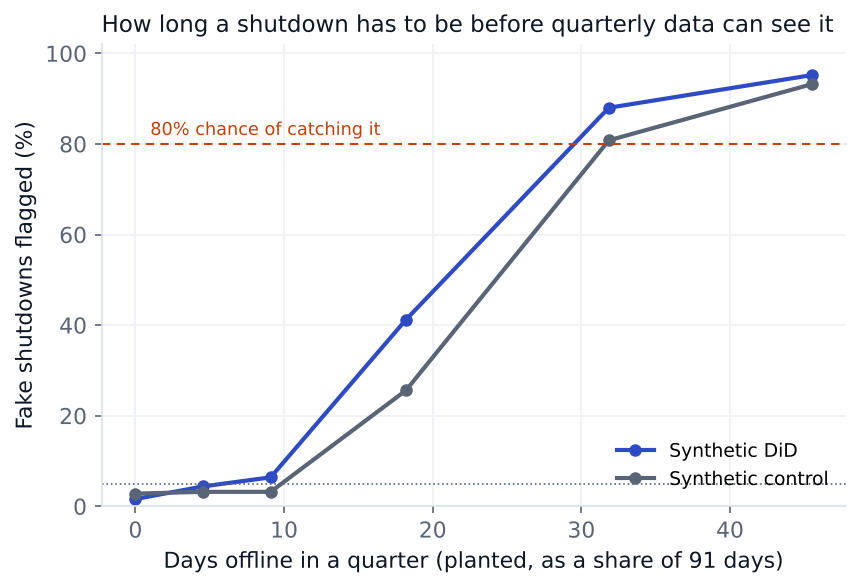
\includegraphics[width=0.6\linewidth]{power.png}
\caption{Share of planted shutdowns flagged at 5\%, 250 per size (version 1 simulations, unchanged).}
\end{figure}

\end{document}
